\chapter{1}
\endgroup

\section{Mailand (IT), Sonntag, 19.
August}



Louis schwitzte. Er wischte sich mit dem Handrücken die Schweissperlen von der Stirn und schaute gedankenverloren aus dem schmalen Küchenfenster. Vielleicht liess sich Liebeskummer messen.
 
Seine Kreationen waren gelungen, einmal mehr, die Gäste zufrieden, das «Ristorante» begehrt und entsprechend dauerausgebucht. Die Mittagsgäste hatten sich nach und nach verabschiedet. Louis freute sich über den frühen Feierabend. Draussen auf der Strasse hatte sich der Verkehr beruhigt. Er holte das Hinweisschild hinein und stellte es beim Eingang in die Ecke. Am Tresen stand Marco. Er zwinkerte Louis zu. Als Zeichen der Wertschätzung, eingespielt über die Zeit und bedeutungsvoll.
Ein Sommerabend lag vor Louis, hitzegeschwängert und trocken. Wie zuvor einige Tage in Folge.

Draussen schlug ihm die Sonne hart entgegen. Unbarmherzig heisser als zu Mittag. Während der wenigen Gehminuten bis zu seiner Wohnung versuchte er, sich den Schatten entlang zu retten.

\sectionbreak

Es war wie jeden Abend und über die Wochen zur Gewohnheit geworden. Ray Charles füllte seine kleine Wohnung mit \emph{«Giorgia»} aus. Louis entkleidete sich und stieg in die Dusche. Grandpère hatte ihm die Tür zur Musik geöffnet, auch die leicht verstaubte zu Ray Charles. Wie nah er ihm war, noch immer. Heute berührte ihn der Gedanke besonders.
 
\emph{«Al cuoco, al cuoco, al cuoco, a Louis»}, hatte er auch diesmal rufen hören. Dazu klatschende Hände, die schneller wurden. Schliesslich hatte ihn Marcos laute, ausgelassene Stimme in die Gaststube geholt.

\emph{«Vieni fuori, fatti vedere, mio grande cuoco»}.\footnote{«Komm nach vorn, zeig dich, mein Küchenchef.»}

Louis verneigte sich und zeigte mit einer ausladenden Bewegung auf seine Kochfreunde links und rechts. Er lachte. Ähnlich wie damals, als er ihr das erste Mal begegnet war. Er hatte mit dem Trockentuch in den Händen im «Ristorante» gestanden. Sie in der Mitte ihrer Freunde gesessen. Giorgia. Ihr Strahlen stach heraus. Er sah einen Rahmen wilder Locken mit geheimnisvollen Augen mittendrin. Giorgias smartes Lächeln liess ihn beinahe taumeln. Dass sie zwischen ihren Schaufelzähnen eine schmale Lücke hatte, wie Ornella Muti, entdeckte er erst später.

Grandpère hatte die Muti verehrt und ihre Zahnlücke geliebt. Louis erzählte es Giorgia an einem Winterabend, während er ihr mit dem Zeigefinger sanft über ihre Lippen strich. Er liebte es, sie zu necken.
Selbst wenn es mit Giorgia vorbei schien und die Hoffnung auf einen Neustart unter einem denkbar schlechten Stern stand, Louis behielt den Song bei sich. Fast war, als brauche er diese Wehmut, die sich wie ein zurückgestossenes Kind immer wieder aufsässig hineindrängte, als müsste er ihren gegenseitigen Versprechen Zeit geben, sich zu verabschieden.

\qrblock{Ray Charles \emph{«Giorgia»}}{media/QR-Codes/004_Giorgia_Ray_Charles_Spotify.png}

Über die letzten Jahre war er präsenter geworden, sein Grossvater. Rückblickend war es Giorgia, die ihn in Louis wieder hatte aufleben lassen. Nach seinen wiederholten Andeutungen hatte sie mehr wissen wollen. Sie wirkte fasziniert. Louis war regelrecht in seine Grandpère-Geschichten hineingefallen, während sie ihm zuhörte. Mit welcher Hingabe er ihn bereits als kleines Kind an seinem musikalischen Schatz teilhaben liess, erzählte er ihr. Auch von seiner Gitarre, die er ihm zum siebten Geburtstag geschenkt hatte und gleichzeitig eine beachtliche Portion Bedeutung. Grandpère, dieser passionierte Musikliebhaber.

\sectionbreak

\indentedblock{Damals. Fribourg, vier.

Louis sitzt neben Grandpère. Auf dem braunen Sofa. Es riecht nach Leder. Sein Grossvater hält ihn im Arm. Es fühlt sich warm an. Sie hören zusammen Musik und reden. Wie oft. Louis liebt es. Er ist gross und wichtig. Sie stellen sich Fragen und versuchen, sie gegenseitig zu beantworten. 
Louis sieht immer wieder zu Grandpère hoch. Sieht das Lachen in seinem Gesicht. 
Ray Charles’ Gesang klingt bis in die hinterste Ecke des Wohnzimmers. Die Töne schweben als bunte Punkte um sie herum. 
Louis ist ganz still, wenn Grandpères Lieblingsmusik läuft. Er darf sich eine Fanta aus dem Kühlschrank holen. Er tut es leise. Hüpfend. Genüsslich saugt er mit dem Trinkhalm das Getränk in sich ein. Die Dose soll nie leer werden.}

\sectionbreak

Das Wasser spritzte scharf aus der Brause und erfrischte Louis’ müden Körper.
Er liebte es, zu kochen und verabscheute zugleich den feuchten, schmierigen Küchengeruch an Haut und Haar. Dieses üble Gemisch aus Fett, Öl und Schweiss, aus Adrenalin und Tempo.
Der Dampf im Badezimmer tat gut. Ein wohlig herber Seifenduft umgab ihn. Er sog ihn tief in sich ein. Er war bereit.

\sectionbreak

Louis packte den Rucksack kurz nach zwanzig Uhr. Aufs Neue überkam ihn die Unsicherheit. Er liess sich aufs Bett fallen.
Der \emph{«Roccia del Culto»}, dieser wundersame Ort auf dem Hügel, über Jahre eine einzige Krafttankstelle, würde wie immer eine Meng Feierfreudiger anziehen. Er ahnte, er würde auch Giorgia begegnen.
Ob er es wirklich wagen sollte, hinzugehen, zu beobachten und auszuhalten, was immer auch geschehen würde? Die Frage beherrschte seine Gedanken, 
selbst wenn er Gemüse schnitt, Fisch briet und Saucen rührte, umgeben von Küche und zwischen seinen Anweisungen an die Gehilfen.

Er setzte sich auf, als ihm ihre gemeinsamen Geschichten weitere Bilder schickten. Erstaunlich klare, direkt und wuchtig. Giorgia und er auf dem Boot. Giorgia tanzend zu seinem Gitarrenspiel. Er mit Giorgia an der Hand und dem Gefühl von Stolz. Sie hatte ihn gross gemacht. Mit Giorgia in Pompeji an Gilmours Konzert. Die Tage in Neapel waren zweifellos einer der Höhepunkte ihrer gemeinsamen Zeit gewesen. Und Louis sah sie beide vor sich, wie sie vor der Bühne gestanden und sich vorgestellt hatten, \emph{«Shine on You Crazy Diamond»} würde nur für sie gespielt.

\qrblock{David Gilmour \emph{«Shine on You Crazy Diamond»}}{media/QR-Codes/005_Shine_On_You_Crazy_Diamond_(Pts._1-5)_Live_At_Pompeii_2016_David_Gilmour_Spotify.png}

Was hatten sie sich nicht alles zu erzählen gewusst, Giorgia und er, stunden - nicht selten nächtelang. 
Wie lebendig er sich in ihrer Gegenwart fühlte. Alles passte.

Die Unstimmigkeiten hatten sich leise angeschlichen. Lange hatte er es geschafft, sie zu ignorieren. Nach und nach waren ihre Diskussionen zu einseitigen Plädoyers von Giorgia verkommen. Und irgend einmal blieb Louis nichts anderes mehr, als die Rolle des sprachlosen Empfängers. Wie auch an diesem 3. Juli, dem Tag, als alles anders wurde. Sie hatte sich aufgesetzt. Angespannt ernst und unmissverständlich gequält hatte sie zu sprechen begonnen, als halte sie eine Trauerrede.

«Ich kann nicht mehr, habe alles versucht. Du bist nicht schuld, Louis. Nein, es liegt bestimmt genauso an mir. Ich liebe dich immer noch, aber anders.»
Ihre Augen hatten sich nach und nach mit Tränen gefüllt. Es schmerzte ihn, sie anzusehen. Sie gestikulierte wild und spürbar verzweifelt, wie nie zuvor.

\begin{figure}[t!]
\centering
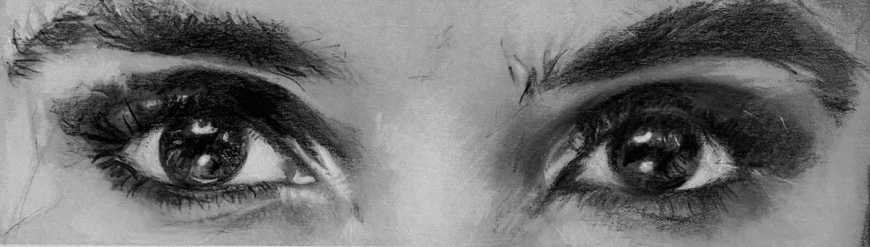
\includegraphics[width=\linewidth,height=!]{media/people/Giorgia.jpeg}
\par
\raggedright\textit{Giorgia Sala}
\end{figure}

«Du bist attraktiv, Louis, umwerfend schön, alles an dir ist schön,» und damit flog ein Funke Licht über Louis’ Gesicht, «bitte schau mich nicht so an, dein, dein Lachen, wenn du glücklich bist, verzeih mir, du musst verstehen, ich kann das Warten nicht mehr aushalten, bis du endlich mal von dir erzählst, ich kann einfach nicht mehr. Es ist mir unmöglich, dich wirklich verstehen zu können.  Als wärst du zwei, als gäb’s dich doppelt. Wenn du Gitarre, Klavier spielst, wenn du singst, Louis, spür ich dich, und dann,» sie wurde leiser und schneller, «hm, der andere Mann ist ein, ein abgeschlossenes Wesen, unerreichbar für mich, ich komme nicht zu dir durch. Ich bring das nicht zusammen, es, es ist vorbei. Wir können Freunde bleiben, gerne, wenn du willst, ich habe es mir anders gewünscht, Louis, den Weg gemeinsam zu gehen, das war mir wichtig. Aber das weisst du alles, nach meinen dauernden Monologen.»

Es war ihr letzter Monolog. Louis sah, wie sich ihre Schultern entspannten. Sie hatte in einem fort gesprochen, einstudiert, schnell und deutlich. Als wollte sie die Worte endlich loswerden. Und Louis hatte, auch zum letzten Mal, stumm und in sich lose vor Schreck, daneben gestanden.
«Ich kann einfach nicht mehr.»
Der entscheidende Satz. Dann war Giorgia weg.
Von nun an kämpfte er. Verlassen und hilflos. 
Die Wut war später dazugekommen.

\sectionbreak

Louis hob die Gitarre vom Bett, nahm sie in die Arme, hielt sie wie eine Geliebte und begann zu spielen, \emph{«Waltzing Matilda»}.
Es sollte wie früher sein. Für diesen Moment. Er sah Giorgia, als stehe sie vor ihm. Sie hatte Rod Stewards Interpretation des Songs geliebt. Louis hatte zu Beginn abgewehrt. Zu emotional sei das, sagte er. Bis sie ihm Herkunft und Hintergrund des Songs erklärt hatte. Von einem in der australischen Wüste wandernden Arbeiter, dem Swagman, hatte sie erzählt, einem Symbol der Liebe zur Freiheit. Nach und nach mochte er den Song. Schliesslich auch, weil die Melodie eins mit Stewarts Stimme und Giorgias Leidenschaft, einen Platz in ihm eingerichtet hatte.

\qrblock{Rod Stewart \emph{«Waltzing Matilda»}}{media/QR-Codes/006_Tom_Trauber's_Blues_(Waltzing_Matilda)_-_2008_Remaster_Rod_Stewart_Spotify.png}

Diese Frau hatte \emph{er} erobern können. Seine Giorgia, wild und ungehalten und frech. Doch auch immer wieder versöhnlich und sanft. Bis vor einigen Monaten. Es tauchten weitere Szenen auf. Drei Jahre zurück. Giorgia hatte neben Louis auf dem Bett gelegen. Als tanzvernarrt hatte sie sich bezeichnet, sich plötzlich aufgesetzt, einen Schluck getrunken und ihm von ihrem ersten Tango-Abend erzählt. Sie konnte sich vor Lachen kaum halten. Um ein Haar hätte sie den Wein verschüttet.

«Der Typ hatte null Rhythmus im Blut und ich war heilfroh, dass die Partner immer wieder wechselten. Ich verstehe ja, dass jeder einen Tanzkurs buchen kann,» sie wurde nachdenklich, «aber bei dem frag ich mich, was das soll.»

Giorgia war direkt hineingeboren worden in eine Welt, die Musik, Körper und Bewegung vereinte. Schon als kleines Mädchen verbrachte sie Stunden und ganze Tage in der Tanzschule ihrer Eltern. Familienzeit hatte sich über die Jahre mehr und mehr in die \emph{Scuola di Danza} verschoben. Giorgia wurde oft sich selbst überlassen, umgeben von den vielen Menschen, die kamen und gingen. Sie hatte ihre Freiheit geliebt und doch jederzeit jemanden gefunden, der für sie da war. Ihre Energie und ihre unbändige Tanzlust hatten ihn immer wieder neu verblüfft. Von Salsa, Cha-Cha-Cha über Rumba bis hin zum Tango konnte er ihre Begeisterung nachvollziehen. Irgendwie. Auch, dass sie sich für die Geschichte der verschiedenen Tanzarten interessierte, alles nachlas, was sie fand und eine Tanzform nach der anderen erfahren wollte. Doch eines Tages wollte sie doch tatsächlich Walzer tanzen, mit ihm. Dann war genug. Er hatte abgelehnt, war irritiert gewesen. Zu lächerlich, fand er, zu fremd für ihn und altbacken. Und eigentlich hatte er sich auch davor gefürchtet, ihr wie ein Tollpatsch auf die Füsse zu treten.

Louis erhob sich und begann ungebremst zwischen Küche und Wohnzimmer hin- und her zu tigern. Die kleine, kompakte Wohnung war übergross und leer geworden. Giorgia fehlte. Am schmalen Küchentisch, ihm gegenüber mit einer Flasche Bier in der Hand, unter der Dusche, während sie ihm etwas zurief; selbst wenn er sich insgeheim nervte, weil er ihre Worte kaum verstand. Oder abends, wenn er spät von der Arbeit nach Hause kam und sie schon schlafend im Bett lag, wo er ihr ihr wildes Haar aus dem Gesicht streichen und sie stumm betrachten konnte.

Nicht nur ihre Kleider, Geschirr und andere Kleinigkeiten hatte sie mitgenommen. Im Bad fehlten auch ihre Frottiertücher. Die grauen, weichen, die ihr so wichtig waren. Der Raum sah verwaist aus. Alleingelassen. Überhaupt, die Wohnung wirkte gleichgültig. Wenn er sich am miesesten fühlte, kamen ihm die zurückgebliebenen Haarklammern, angerissenen Kaugummipäckchen, zu Stummeln gespitzten Kajalstifte und anderer Kleinkram wie Schlachtabfälle vor. Wenn er sich hingegen in Erinnerungen gemeinsamen Glücks wähnte, wurden die Gegenstände zu seinen kleinen Kostbarkeiten.

\sectionbreak

Mit Blick in die Gasse blieb er vor dem Fenster stehen. Er schaute der gegenüberliegenden Fassade entlang nach unten und sah zwei junge Frauen auf einer Vespa vorbeiflitzen. Die Hintere rief der Fahrerin etwas zu. Mit lauter Stimme, mitten in den Motorenlärm des Rollers. Ihre Heiterkeit stieg zu ihm empor, als mache sie sich über ihn lustig. Louis schüttelte den Kopf. Sie verschwanden so rasch, wie sie heran geknattert gekommen waren und gaben der schmalen Nebenstrasse ihre Stille zurück.

\sectionbreak

Louis` Begeisterung für ihre gemeinsamen Tanzaktionen hatte sich schrittweise verabschiedet. Giorgias Vorträgen hingegen hörte er nach wie vor vergnügt zu. Wie so oft hatte er sich auch damals, an diesem saukalten Winterabend im Dezember, auf ihre Erklärungen eingelassen.

«Wusstest du, der erste Walzer ist im 18. Jahrhundert aufgetaucht. Das war verrückt. Hab ich nachgelesen. Stell dir vor, das war der erste Tanz, bei dem Mann und Frau sich körperlich nah kamen, nach diesen distanzierten Menuett-Tänzen.»

Sie hatte die Augen gerollt, sich in die Decken und näher an Louis gekuschelt.

«Die lagen sich wie nie zuvor in den Armen. Diese neue Tanzform hatte in der Gesellschaft damals einen Aufschrei provoziert, das gehöre verboten, sei eine sittliche Beleidigung.»

Giorgia kringelte sich vor Lachen .

«Ach, komm, diese Empörung war vorgetäuscht. Ich will nicht wissen, wie das damals zugegangen ist,» sie schüttelte den Kopf, «im Versteckten, mein ich.»

Louis hatte in ihre Augen gesehen. Er beobachtete sie zärtlich und genau. Es war nicht der Inhalt ihrer Erzählung, der ihn packte. Es war sie und dieser grenzenlose Enthusiasmus. Eigentlich schenkte ihm ihre Lebensart willkommene Momente der Leichtigkeit. Giorgia hatte sich hastig eine Locke aus dem Gesicht gestrichen und fuhr aufgekratzt fort.

«Ich rede natürlich vom richtigen Walzer im Dreiviertel-Takt, und da hat Rod Stewart bei «Waltzing Matilda» den Takt verfehlt. Also, Rod Stewart, stimmt ja eigentlich nicht, der Song ist ursprünglich von Tom Waits, aber egal, ich mein, klar, der Song ist wunderschön, aber die Worte machen doch noch keinen Walzer, oder?»

Seine Antwort wartete sie nicht ab. Sie holte Luft und ein Strahlen legte sich über ihr Gesicht.

«Aber dass ich Cohens \emph{«Take This Waltz»} entdeckt habe, wow, ist der Knüller. Das ist ein richtiger Walzer und Maria hat recht, Cohens Stimme und seine Ausstrahlung sind im Alter immer noch besser geworden. Das war vielleicht ein würdevoller Typ. Dem wär ich gern mal begegnet.»

Dabei hatte sich Louis klein gefühlt.

\qrblock{Leonard Cohen \emph{«Take This Waltz»}}{media/QR-Codes/007_Take_This_Waltz_-_Paris_Version_Leonard_Cohen_Spotify.png}

Immer wieder sah er sie vor sich, Giorgia, dieses reiche Paket an Leidenschaft, Überraschung und Kraft.
Lange hatte es funktioniert, hatte er seine Sprachlosigkeit mit Charme wettgemacht. Wenn ihm die Worte fehlten. Wenn er vor seinen Barrieren stand. Wenn er verstummte, sobald sie mehr von ihm wissen wollte. Wie oft hatte er wie ein Gefangener nach rettenden Einfällen gesucht, sich als leer empfunden und war konsequent ausgewichen. Parallel zu Louis’ Überforderung hatte sich Giorgias Geduld abgenutzt. Sie war hartnäckiger, gelegentlich auch lauter und kompromissloser geworden.

\sectionbreak

Er fühlte sich weit mehr als einsam. Er war verloren. 

Louis’ Herz pumpte sich mit unbändiger Wehmut auf und ein Schleier Wut legte sich über seine Traurigkeit. Es fühlte sich an, als würden sich seine Tränen hinter den Augen zu Stauseen aufsammeln. Wie lange würden die Schleusen dem Druck noch standhalten?

Wer war er eigentlich?

Er schleppte sich zurück ins Schlafzimmer, setzte sich auf die Bettkante, griff seine Gitarre und spielte vor sich hin. Die ersten Klänge beruhigten ihn. Mit dem letzten Akkord schrak er zusammen, sass da wie zuvor, und nichts war anders. Solche Momente waren zu aufgezwungenen Verbündeten geworden. Tröstlich wenigstens, dass sich seine Verzweiflung auf ihrem Höhepunkt früher oder später zu wandeln vermochte und zu Entschlossenheit wurde. Wie jetzt. Er erhob sich, schulterte seinen Rucksack, packte die Gitarre in den Koffer, richtete sich gerade auf und schloss mit einer kräftigen Schlüsseldrehung hinter sich ab. Es war kurz vor einundzwanzig Uhr.

Das Klicken seiner Schuhe gab der leeren Gasse eine gespenstische Note. Es erinnerte ihn an das Ticken einer Zeitbombe.
Die Tageshitze hatte sich unterdessen zu Boden gelegt. Der komprimierte Duft des Spätsommers drückte. Louis schritt den mächtigen, dicht aneinander gereihten Bäumen auf der \emph{Corsa} entlang. Bunt gekleidete Menschen waren auf den Gehsteigen unterwegs. Er ging langsam.
 
Schliesslich erreichte er die \emph{Piazza 5 Giornate.} 
Als er die Treppe zur Metro hinunterstieg, fragte er sich erneut, ob es wirklich klug war, wieder hochzugehen. Nach all den Wochen?
Die Metro war brechend voll. 
Louis stellte den Gitarrenkoffer auf seinen Schuhspitzen ab. Er atmete flach.
